\documentclass[12pt]{article}

\usepackage{fullpage}
\usepackage{graphicx, rotating, booktabs} 
\usepackage{times} 
\usepackage{natbib} 
\usepackage{indentfirst} 
\usepackage{setspace}
\usepackage{grffile} 
\usepackage{hyperref}
\usepackage{adjustbox}
\setcitestyle{aysep{}}


\singlespace
\title{\textbf{Appendix: Trump and Public Support for Democracy Abroad}}
%\author{Joshua Alley and John Owen} 
\date{}

\bibliographystyle{apsr}

\begin{document}

\maketitle 

\singlespace 

This appendix provides more detail about the multilevel model in the manuscript and association between the Trump administration and democratic support in Asia. 
Please note that the World Values survey does not permit disseminating copies of the data in replication archives. 
We used version 1.6 of the World Values survey longitudinal data, which can be downloaded from: \url{https://www.worldvaluessurvey.org/WVSDocumentationWVL.jsp}.



\section{Model Specification} 



The varying slopes model lets the relationship between U.S. success and other year-level factors shift across regions, rather than assuming a constant effect. 
The binomial likelihood of the proportion of high democratic support given the number of respondents within each state-year group can be expressed as follows, with the probability of success $\theta$ for each country-year observation partially pooled such that ~ $\theta_i \sim N(\mu_i, \sigma)$ : 


\begin{equation}
\mathrm{ y \sim Binomial(Num. Resp, \theta_i)}
\end{equation} 

The expected value of high democratic support $\mu$ in each state-year observation is:

\begin{equation}
\mathrm{ \mu = \alpha + \alpha_{state} + \alpha_{year} + \textbf{X} \beta + \textbf{Z} \gamma +  \textbf{G} \lambda_{region}} 
\end{equation} 

There are three sets of variables here. 
The year level variables matrix $\textbf{G}$ has varying slopes by region.
The state level variables $\textbf{Z}$ and $\textbf{X}$ do not change across regions. 


The specification subsumes regional intercepts and year varying slopes expressed in $\textbf{G}$ into a multivariate normal prior with covariance matrix $\Sigma$ with an LKJ prior, further optimized with a Choleskey factorization: 

\begin{equation}
\mathrm{\alpha_{region}, \lambda_{region} \sim \mbox{multivariate normal}(\mu_{region}, \mu_{\lambda}, \Sigma)}
\end{equation}
 

\autoref{tab:priors} summarizes the other prior distributions in the multilevel model. 
All priors are weakly informative relative to the scale of the data, and the regression parameters are robust to unusually large effect sizes. 
We employ non-centered parameterizations of the state and year intercepts in fitting the model. 



\begin{table} % Create a table of priors.
\begin{center}
\begin{tabular}{c} 
$ p(\alpha) \sim N(0, 1)$  \\
$ p(\alpha_{year}) \sim N(G \lambda, \sigma^{yr}) $ \\ 
$ p(\sigma^{yr}) \sim \mbox{half-}N(0, 1) $ \\
$ p(\alpha_{state}) \sim N(\mu_{state}, \sigma^{st}) $ \\ 
$ p(\mu_{state}) \sim N(0, 1) $ \\ 
$ p(\sigma^{st}) \sim \mbox{half-}N(0, .5) $ \\ 
$ p(\beta) \sim \mbox{student-t}(5, 0, 1) $ \\
$ p(\gamma) \sim \mbox{student-t}(5, 0, 1) $ 
\end{tabular} 
\caption{Summary of Priors in Multilevel Model} 
\label{tab:priors}
\end{center} 
\end{table} 





\section{Hamiltonian Monte Carlo Diagnostics}

We fit these models with STAN \citep{Carpenteretal2016}.
There were no divergent iterations in either sample running 4 chains for 2,000 iterations with 1,000 warmup iterations in any of the imputed datasets.  
The split $\hat{R}$ statistic is less than 1.1 for all parameters as well.
Energy diagnostics and the effective sample size for the potsterior medians and tails were also satisfactory.  
All of these estimates suggest that the Hamiltonian Monte Carlo adequately explored the posterior distribution. 


\section{Variables}


This section summarizes the key variables in the model. 
The state and individual level variables account for other determinants of attitudes towards democracy. 
State-year variables include income inequality, GDP levels and growth, financial crisis presence, liberal democracy, human rights practices, civil war deaths, U.S. aid disbursements and globalization. 
We use the VDEM measure of democracy for the U.S. and other states as it is a common measure of democratic quality \citep{WaldnerLust2018}.
We control for U.S. aid disbursements to ensure that our leadership findings do not reflect changes in investment in democracy promotion and aid more generally.\footnote{Data on U.S. democracy promotion aid has unfortunate temporal limitations.} 
We also adjust for individual political ideology, perceptions of domestic political institutions, and economic security.


In the remainder of this section, we tabulate the variables at each level of analysis. 
We start with the year-level variables that measure U.S. success and failure. 
\autoref{tab:year-vars} summarizes these variables and their distribution. 
\autoref{tab:state-vars} summarizes the state-level variables across all imputed datasets.
Last, \autoref{tab:wvs-vars} shows summary statistics for the individual level variables in the analysis, which are averaged at the state year. 
It also includes the distribution of high democratic support sums and the number of respondents, which are the key quantities in the binomial proportions.
 
 
\begin{table}
\caption{\label{tab:year-vars}Year Level Variables}
\centering
\begin{tabular}[t]{lrrrrrrr}
\toprule
  & Unique (\#) & Missing (\%) & Mean & SD & Min & Median & Max\\
\midrule
US GDP Growth & 29 & 0 & 2.58 & 1.66 & -2.54 & 2.68 & 4.75\\
US Democracy & 23 & 0 & 0.80 & 0.03 & 0.74 & 0.80 & 0.86\\
US Human Rights & 29 & 0 & 0.73 & 0.68 & -0.17 & 0.55 & 1.88\\
US Protests & 29 & 0 & 0.69 & 0.17 & 0.42 & 0.72 & 1.05\\
US GINI & 22 & 0 & 36.72 & 1.93 & 31.60 & 37.40 & 38.50\\
Clinton & 2 & 0 & 0.21 & 0.41 & 0.00 & 0.00 & 1.00\\
W.Bush & 2 & 0 & 0.28 & 0.45 & 0.00 & 0.00 & 1.00\\
Obama & 2 & 0 & 0.24 & 0.44 & 0.00 & 0.00 & 1.00\\
Trump & 2 & 0 & 0.07 & 0.26 & 0.00 & 0.00 & 1.00\\
Chinese Growth & 29 & 0 & 9.02 & 2.45 & 3.91 & 9.23 & 14.23\\
US Intervention & 3 & 0 & -0.10 & 0.56 & -1.00 & 0.00 & 1.00\\
\bottomrule
\end{tabular}
\end{table}



\begin{table}
\caption{\label{tab:state-vars}State Level Variables}
\centering
\begin{tabular}[t]{lrrrrrrr}
\toprule
  & Unique (\#) & Missing (\%) & Mean & SD & Min & Median & Max\\
\midrule
GDP per Capita & 250 & 0 & 14181.60 & 16819.63 & 273.49 & 7563.99 & 91565.73\\
GDP Growth & 248 & 0 & 4.37 & 5.47 & -24.00 & 4.10 & 54.16\\
Information Flow & 233 & 0 & 64.42 & 19.17 & 13.28 & 68.37 & 94.82\\
Social Globalization & 233 & 0 & 59.52 & 18.65 & 12.00 & 61.37 & 90.81\\
Bank Crisis & 2 & 0 & 0.09 & 0.29 & 0.00 & 0.00 & 1.00\\
Liberal Democracy & 216 & 0 & 0.49 & 0.27 & 0.03 & 0.50 & 0.89\\
Conflict Battle Deaths & 29 & 0 & 462.40 & 3189.60 & 0.00 & 0.00 & 35071.00\\
Human Rights & 236 & 0 & 0.11 & 1.52 & -2.57 & -0.02 & 3.97\\
Inequality & 157 & 0 & 37.45 & 9.05 & 17.50 & 36.90 & 63.20\\
U.S. Aid & 145 & 0 & 281572388.69 & 963425070.89 & 6251.00 & 46748184.00 & 10149892020.00\\
\bottomrule
\end{tabular}
\end{table}



\begin{table}
\caption{\label{tab:wvs-vars}Individual Level Variables}
\centering
\begin{tabular}[t]{lrrrrrrr}
\toprule
  & Unique (\#) & Missing (\%) & Mean & SD & Min & Median & Max\\
\midrule
Sum: High Democ. Support & 1147 & 0 & 676.14 & 324.14 & 76.00 & 627.50 & 1689.00\\
Avg: Political Interest & 2262 & 0 & 2.68 & 0.31 & 1.27 & 2.72 & 3.38\\
Avg: Country Aim & 2956 & 0 & 1.74 & 0.25 & 1.23 & 1.73 & 2.62\\
Avg: Left or Right & 4471 & 0 & 5.81 & 0.60 & 2.77 & 5.79 & 8.93\\
Avg: Government Confidence & 3048 & 0 & 2.65 & 0.38 & 1.26 & 2.72 & 3.44\\
Avg: Rate Political System & 4628 & 0 & 5.07 & 0.74 & 2.38 & 5.13 & 8.60\\
Avg: Nationalism & 3752 & 0 & 0.19 & 0.10 & 0.00 & 0.17 & 0.45\\
Avg: Financial Satisfaction & 3289 & 0 & 5.71 & 0.98 & 3.06 & 5.91 & 8.21\\
Avg: Respect Authority & 2577 & 0 & 0.27 & 0.17 & 0.02 & 0.23 & 0.89\\
Number of Respondents & 170 & 0 & 1450.53 & 574.91 & 240 & 1216.00 & 4078\\
\bottomrule
\end{tabular}
\end{table}


\section{Other Estimates}


This section of the appendix summarizes other estimates from the multilevel model in the manuscript. 
First, we describe estimates from the state and individual level variables in \autoref{fig:other-levels-vars}. 
Then we plot the estimated probability of robust democratic support across post Cold War presidents in \autoref{fig:theta-est}. 


\begin{figure}
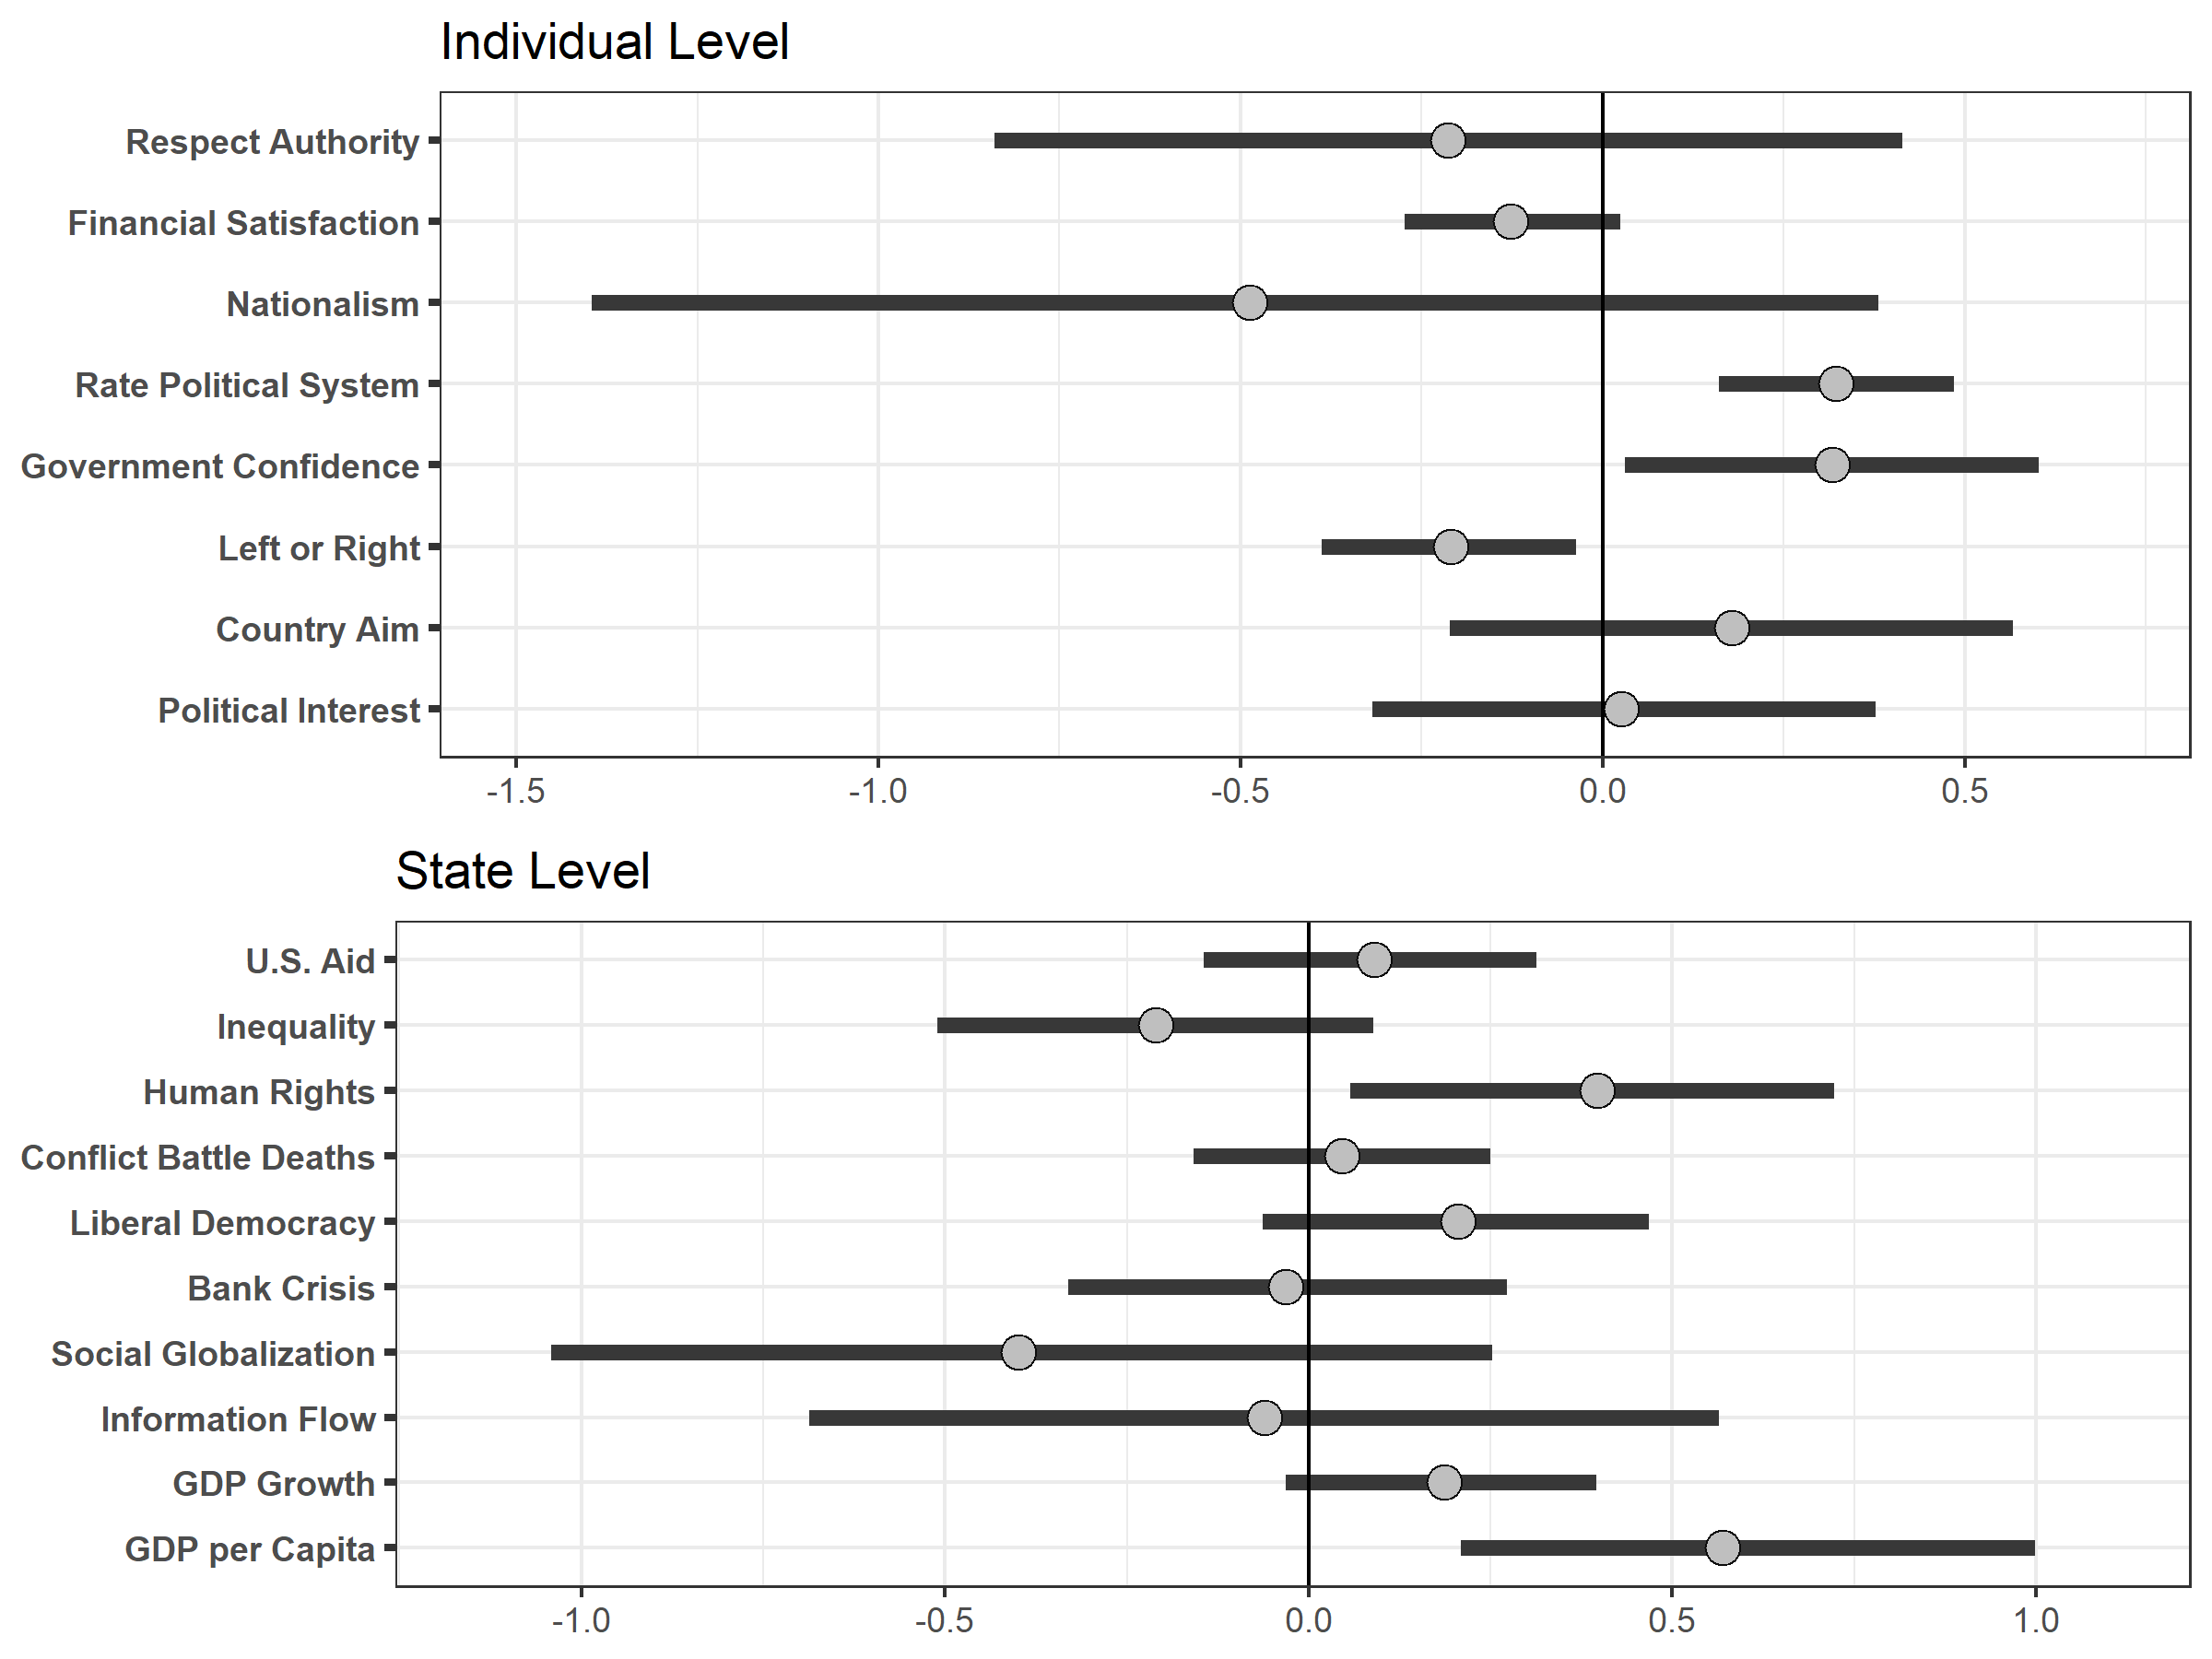
\includegraphics[width = .95\textwidth]{other-levels-vars.png}
\caption{Estimated association between individual and state level variables and the probability of high democratic support. Point estimates mark the posterior median, and error bars summarize the 90\% credible interval.}
\label{fig:other-levels-vars} 
\end{figure}


Some individual and state-level variables also impact support for democracy outside the United States. 
The individual variables are averaged at the country-year level to facilitate binomial model fitting, as the individual estimates compare averages across state-year estimates.
Higher average ratings of the political system and confidence in the government in a country increase the likelihood of high democratic support. 
Countries where individuals are more right-wing on average express lower support for democracy. 
The nationalism and financial satisfaction averages are also negative, but are more uncertain.


At the state level, GDP per capita and respect for human rights are positively associated with high democratic support. 
The GDP growth and liberal democracy coefficient estimates are largely positive, but consistent with slight negative effects. 
The income inequality and social globalization coefficients are mostly negative with substantial uncertainty. 


\begin{figure}
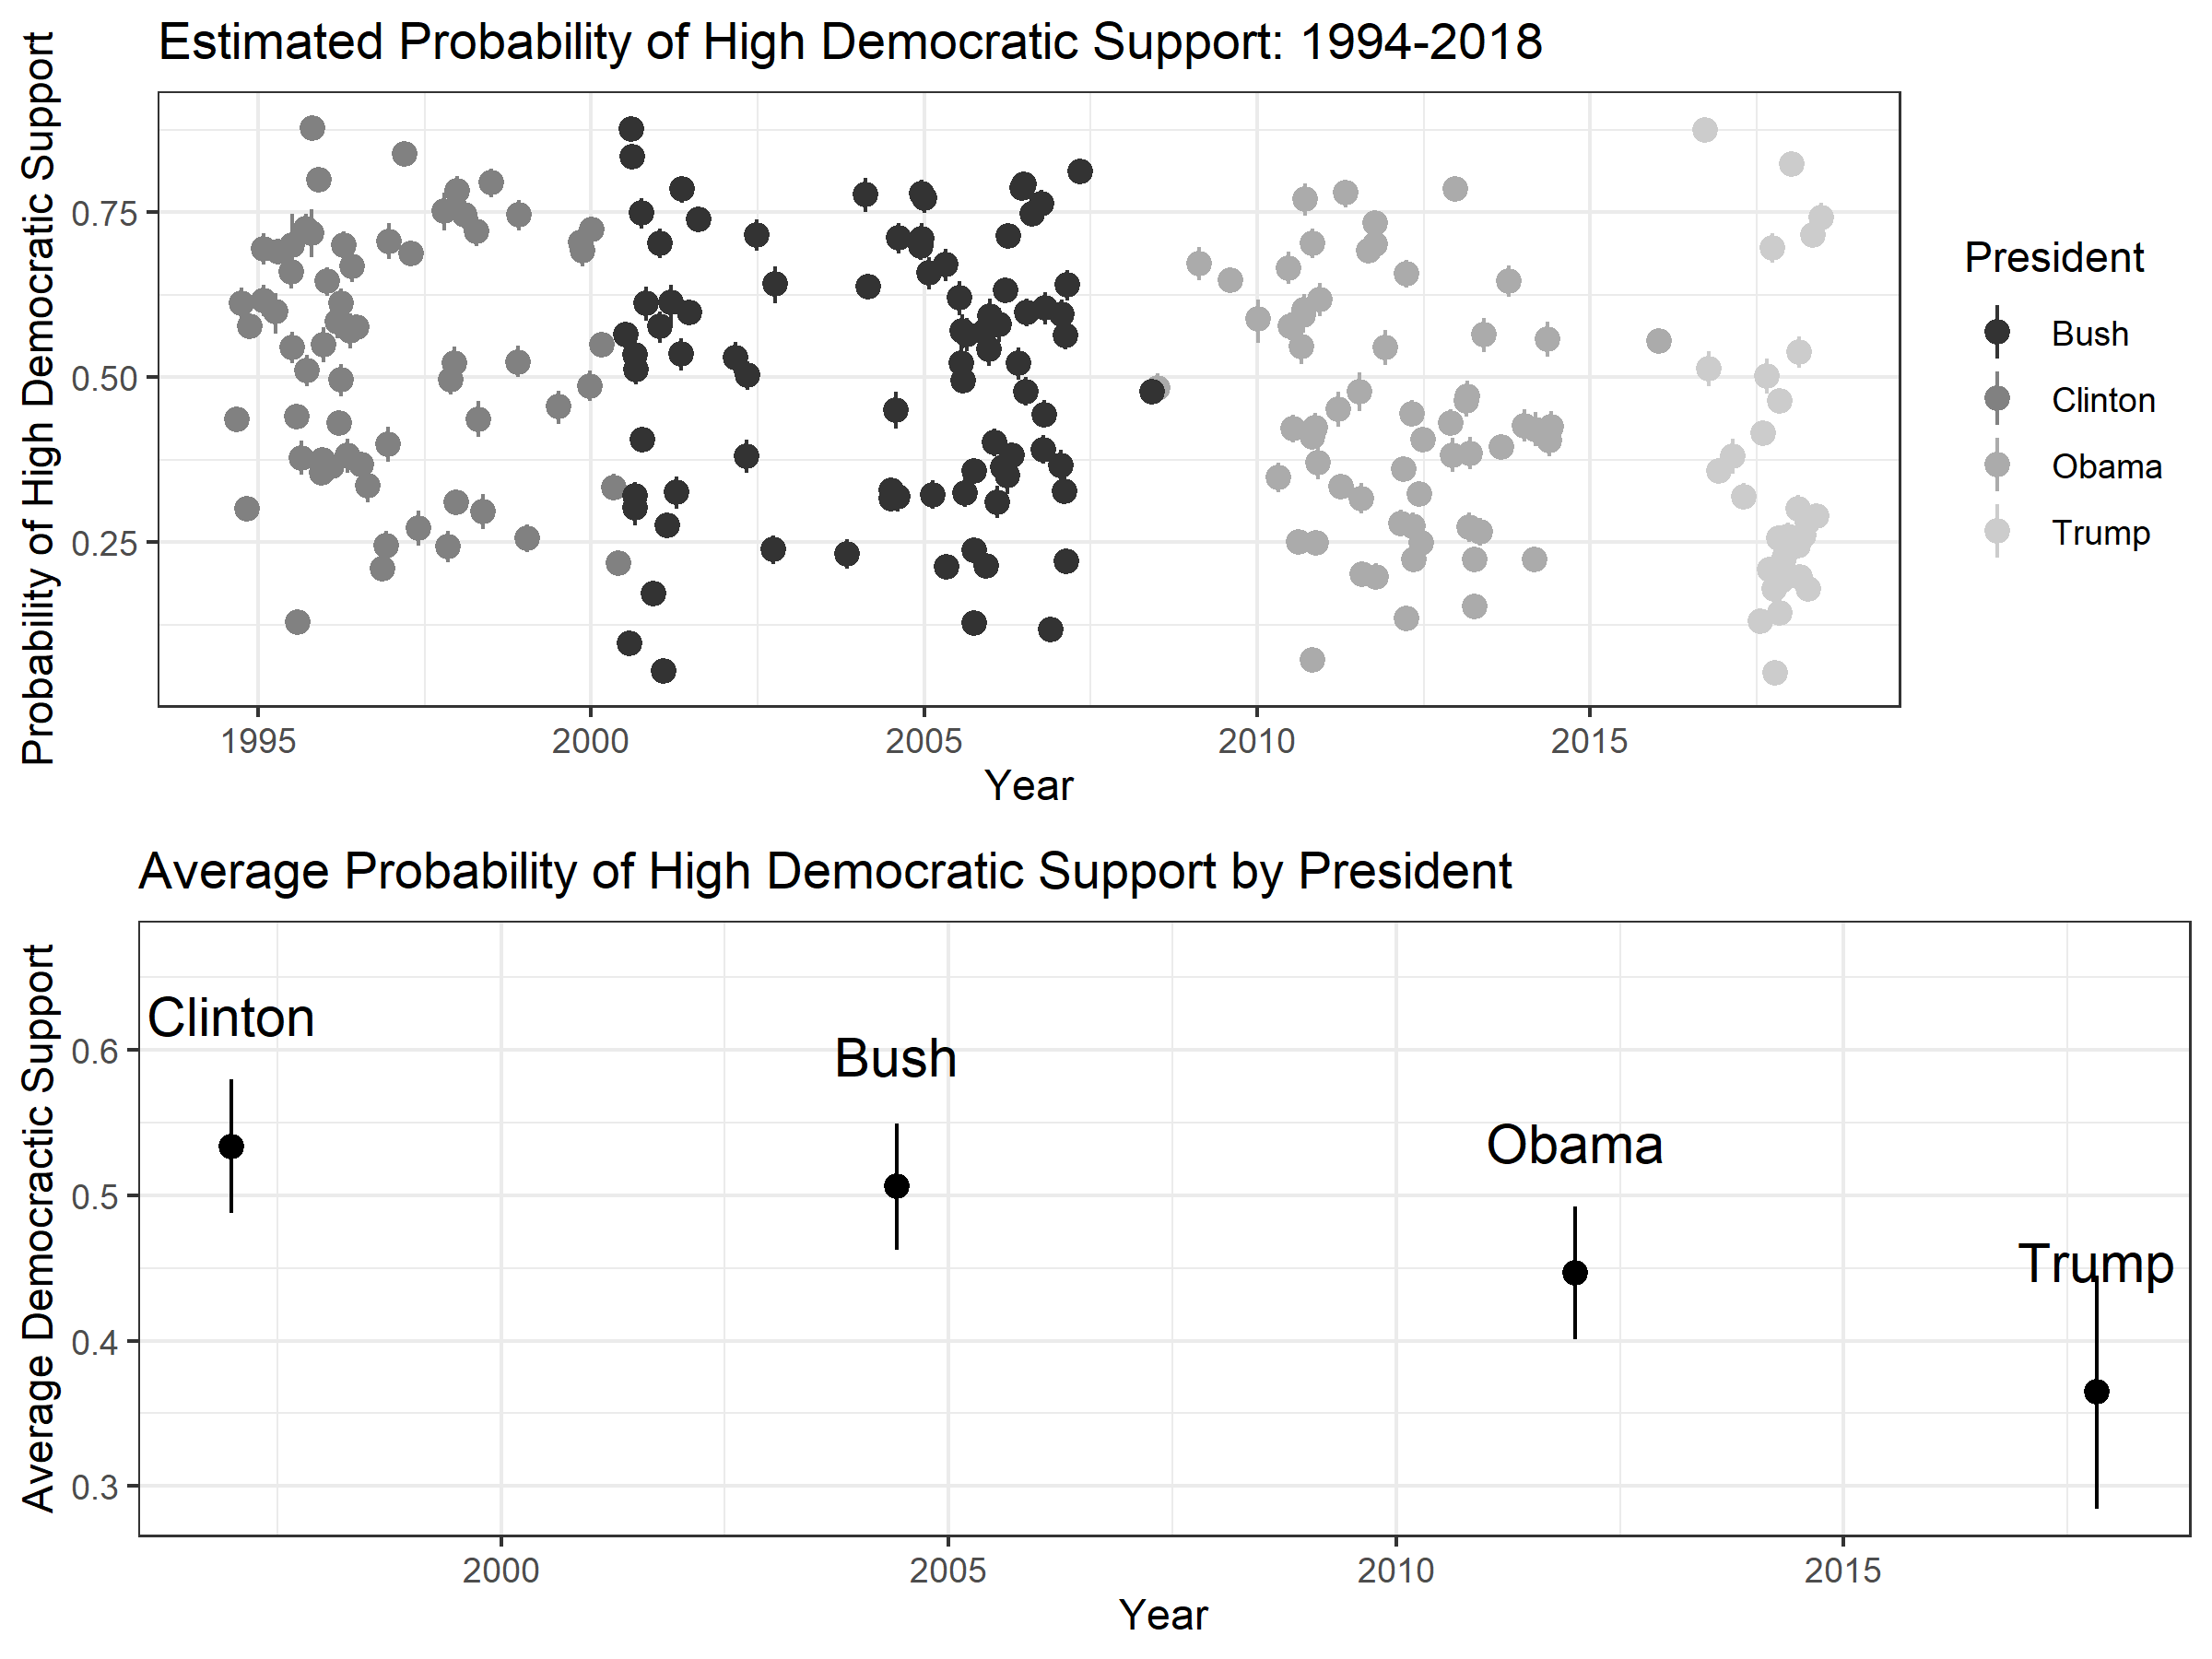
\includegraphics[width = .95\textwidth]{theta-est.png}
\caption{Estimated probability of high democratic support in country-year observations from 1994 to 2018, with averages by presidential administration. In the top panel, each point marks the estimated probability of high democratic support in a country-year observation, and the error bars summarize the 90\% credible interval. The bottom panel is the average of the posterior medians for each president. Estimates from before 1994 omitted to make the plot more legible.  }
\label{fig:theta-est} 
\end{figure}


\autoref{fig:theta-est} plots the estimated probability of high democratic support for each country-year observation in the WVS from 1994 to 2018. 
Each point is the estimated $\theta$ parameter in the binomial logit model.
This is the probability of a success ---high democratic support--- in the number of binomial trials given by the number of respondents. 


There are some notable patterns in democratic support over time.
The first is that the average of the $\theta$ parameters by President declines gradually over time, before dropping dramatically during the Trump administration.  
This is driven by a cluster of state-year observations with very low probabilities of high democratic support. 
Interestingly, several estimates from the Trump administration are higher than any from the Obama administration. 
Further data might show global polarization in democratic support. 


\section{Trump and Democratic Support in Asia}

The models in the manuscript find a negative impact of the Trump administration on support for democracy in Asia. 
In this section of the appendix, we explore that finding further. 
To do so, we fit separate models to each state in Asia that had WVS data before and after Trump took office in early 2017. 
This generates results for nine countries. 


Fitting separate models for each state is a simple way to assess whether the impact of the Trump administration and other factors varies by country. 
It also allows us to draw on the full range of the democratic support variable, instead of simplifying it to a dummy, as in the manuscript. 
Because democratic support takes on relatively few integer values, we fit Bayesian ordinal logit models with flexible thresholds between the outcome levels using BRMS \citep{Buerkner2017}.
The lack of cross-sectional variation in these analyses meant we could only include two state and year level variables without introducing perfect multicollinearity into the model. 
We therefore included a national economic growth variable and the Trump administration dummy, in addition to a series of controls at the individual level. 
For each state, we fit models to five imputed datasets, and then combined them into a single posterior, following standard practice. 


We find that the Trump presidency reduced support for democracy throughout Asia. 
\autoref{fig:asia-state-trump} plots the estimated coefficient on the Trump administration dummy variable from each of the nine models of democratic support over time in Asia states. 
Most of the coefficient estimates are negative, and most are substantively large as well. 


\begin{figure}
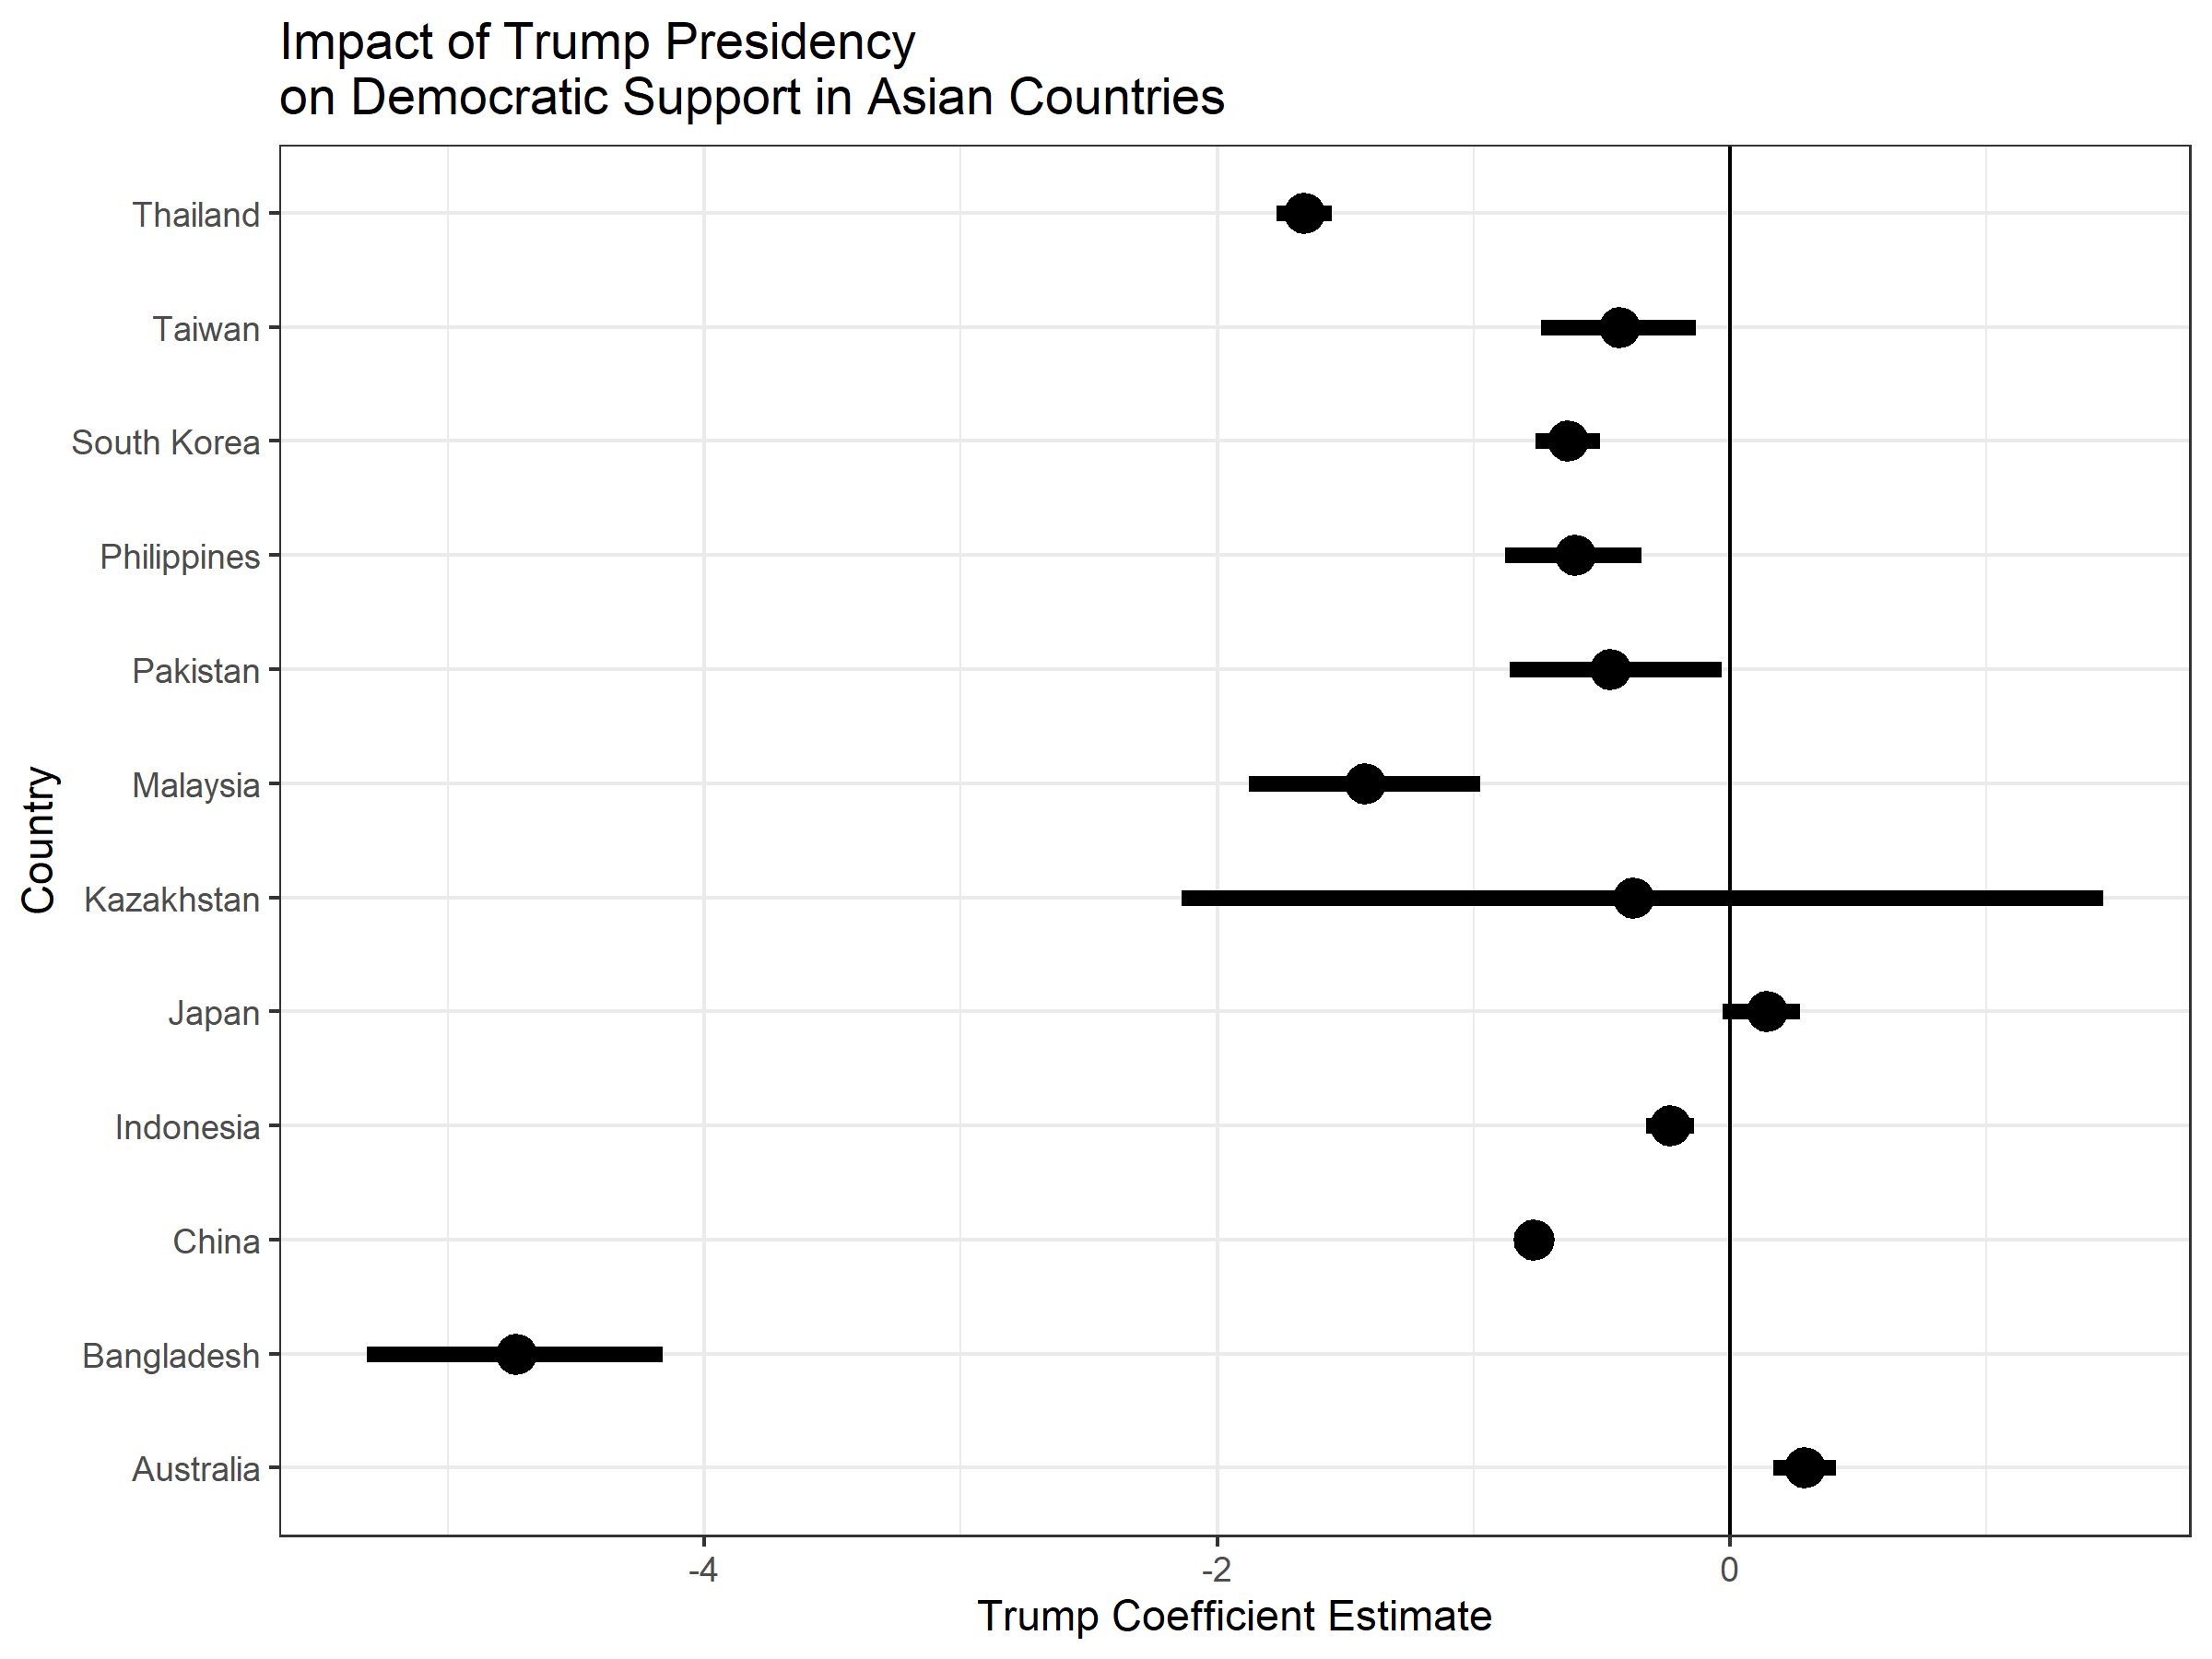
\includegraphics[width = .95\textwidth]{asia-state-trump.png}
\caption{Estimated association between Donald Trump's presidency and public support for democracy in nine Asian countries, 1980 to 2019. Point estimates mark the posterior median, and error bars summarize the 90\% credible interval.}
\label{fig:asia-state-trump} 
\end{figure}


The Trump effect is largest in Bangladesh, but the coefficient magnitude may reflect that only three WVS waves covered Bangladesh, so there is limited temporal variation in that model. 
The Kazakhstan coefficient has substantial uncertainty for similar reasons. 
Only in Australia is the Trump administration correlated with increased democratic support. 


Indonesia, Thailand, South Korea, Pakistan, Malaysia and China all saw lower public support for democracy during the Trump administration. 
The common change in a group with such varied characteristics implies that a common shock is plausible. 
The mechanism likely differs across these countries, however. 
South Korea is a close U.S. ally, and Thailand is somewhat aligned with the United States.
China's relationship with the Trump administration was often antagonistic. 
Pakistan has some ties to the U.S., along with close connections to China. 
  
  
  \newpage
\bibliography{../../MasterBibliography} 




\end{document}
